\chapter{The Inhabited Library}

\vspace{1em}
\hfill
\begin{minipage}[c]{0.55\textwidth}
\raggedleft
\small\itshape
The world is everything that is the case.\\[0.5em]
\upshape\footnotesize Ludwig Wittgenstein, \textit{Tractatus Logico-Philosophicus} (1921)
\end{minipage}%
\hspace{0.5em}
\begin{minipage}[c]{0.12\textwidth}
% \includegraphics[width=\textwidth]{figures/ch07_inhabited.png}
\end{minipage}
\vspace{1.5em}

\noindent \textsc{Chapter 6 exposed the slip.} The universal semimeasure weights candidate programs and output prefixes. Turning those weights into a measure on realities would require an additional ontological choice, and the book holds that choice open.

What follows are the two pictures now available, an older question they sharpen, and the honest limits of either.

\section*{What the postulate gives, and does not}

With the postulate taken, no decomposition is view-independently privileged. From there, two pictures remain.

In Picture A, program-output space is contemplated as a total object. In Picture B, you are situated with finite data and a posterior over candidate programs. In both pictures, $M$ weights programs whose outputs begin with your data. It does not establish that every output is a real world.

Your current data can be compatible with many programs: some encode simple lawful histories, some stranger continuations, some a momentary matching state. That is ordinary Bayesian underdetermination. It does not yet follow that each match is an observer occurrence, that each occurrence exists, or that $M$ gives proportions among occurrences.

\begin{figure}[h]
\centering
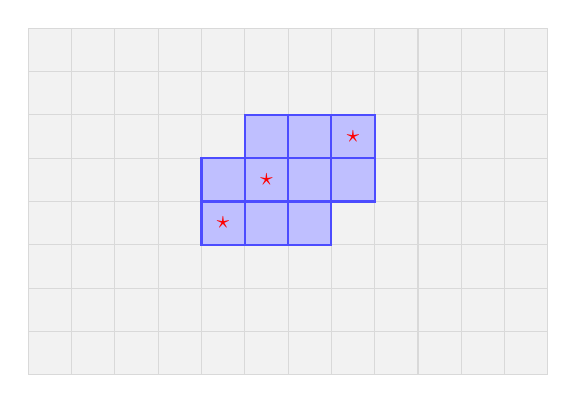
\begin{tikzpicture}[scale=0.55]
  % Schematic candidate descriptions
  \foreach \x in {0,1,...,11} {
    \foreach \y in {0,1,...,7} {
      \draw[gray!30, fill=gray!10] (\x, \y) rectangle ({\x+1}, {\y+1});
    }
  }

  % Candidate descriptions consistent with your data (blue cells)
  \foreach \x/\y in {4/3, 5/3, 6/3, 4/4, 5/4, 6/4, 7/4, 5/5, 6/5, 7/5} {
    \draw[thick, blue!70, fill=blue!25] (\x, \y) rectangle ({\x+1}, {\y+1});
  }

  % Mark possible observer occurrences without weights
  \foreach \x/\y in {4/3, 5/4, 7/5} {
    \node[font=\small\bfseries, red] at ({\x+0.5}, {\y+0.5}) {$\star$};
  }
\end{tikzpicture}
\caption{Membership only. Gray cells schematically represent candidate program descriptions; blue cells are consistent with your data; red stars mark possible observer occurrences under an ontic reading. Equal cell sizes carry no counting or probability claim. $M$ weights candidate programs, not the stars. A distribution over occurrences requires an additional self-location rule.}
\label{fig:multiplicity}
\end{figure}

The question \emph{where am I?} now splits. Which programs best predict my next data? $M$ supplies a posterior answer, relative to $U$. Which observer occurrence is me? The framework has not yet defined the sample space or a distribution. That second question is open, not merely diffuse.

\section*{A note on time}

A reader will want to ask about time. Picture A presents program-output space statically; but the universe you inhabit plainly has time in it, change, before and after, a present that seems to move. How can a static description represent that?

One can represent an execution by its complete trace, indexed by a step counter. Step $5$ and step $6$ are both parts of that mathematical object. On the block-universe analogy, ``running'' is the embedded order in which configurations relate, not a motion of the whole representation. This is a feature of Picture A, not a result that settles the metaphysics of time.

\section*{An older question}

A reader who has followed this far may have an older question waiting. \emph{Why is there something rather than nothing?}

The question seems to assume that nothing is the simpler option. The chapter's tools do not directly settle this. Nothing, taken seriously, is the empty set: every possibility excluded. Like the universal set, it is informationally cheap. Both extremes have low description length. They are, in a sense, complements of the same kind of thing.

\begin{figure}[h]
\centering
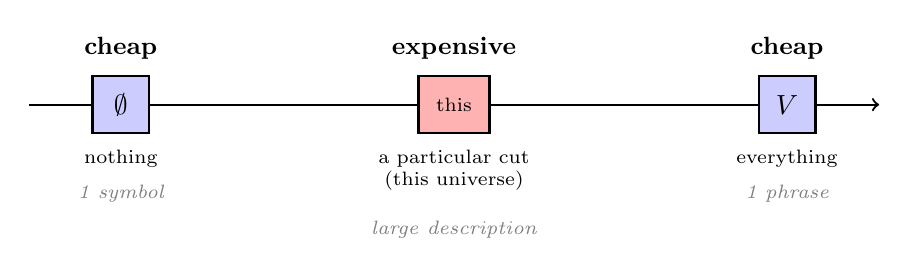
\begin{tikzpicture}[scale=0.9]
  % Horizontal axis line
  \draw[->, thick] (0, 0) -- (12, 0);

  % Position 1: ∅ (left end)
  \draw[thick, fill=blue!20] (0.9, -0.4) rectangle (1.7, 0.4);
  \node[font=\normalsize] at (1.3, 0) {$\emptyset$};
  \node[font=\scriptsize, anchor=north] at (1.3, -0.5) {nothing};
  \node[font=\scriptsize\itshape, gray, anchor=north] at (1.3, -1) {1 symbol};

  % Position 2: this universe (middle)
  \draw[thick, fill=red!30] (5.5, -0.4) rectangle (6.5, 0.4);
  \node[font=\scriptsize, align=center] at (6, 0) {this};
  \node[font=\scriptsize, anchor=north, text width=3.5cm, align=center] at (6, -0.5) {a particular cut (this universe)};
  \node[font=\scriptsize\itshape, gray, anchor=north] at (6, -1.5) {large description};

  % Position 3: V (right end)
  \draw[thick, fill=blue!20] (10.3, -0.4) rectangle (11.1, 0.4);
  \node[font=\normalsize] at (10.7, 0) {$V$};
  \node[font=\scriptsize, anchor=north] at (10.7, -0.5) {everything};
  \node[font=\scriptsize\itshape, gray, anchor=north] at (10.7, -1) {1 phrase};

  % Top labels
  \node[font=\small\bfseries] at (1.3, 0.8) {cheap};
  \node[font=\small\bfseries] at (6, 0.8) {expensive};
  \node[font=\small\bfseries] at (10.7, 0.8) {cheap};
\end{tikzpicture}
\caption{The endpoints and the cut. The empty set and the universal set are both informationally cheap, describable in a phrase. A specific intermediate cut (such as ``this particular universe'') requires substantial information. The cost lives in the cut, not in the totality. Nothing and everything are, by this measure, on equal footing.}
\label{fig:endpoint-spectrum}
\end{figure}

So the cut principle does not, by itself, favor either nothing or something. Both are cheap.

What does favor something: we observe it.

You are reading these words. Something exists. This is not a metaphysical assumption; it is the data. Any theory of reality that predicts no existence at all is immediately falsified by the existence of the observer. The nothing-hypothesis is excluded by induction on the only sample available, which is the entirety of what anyone has ever observed.

This is thinner than the inductions of earlier chapters. The fact of experience contradicts the proposition that there is no experience at all. It does not identify a generator, select Picture A, or supply a probability distribution over ontologies.

There is also a coherence question. Is \emph{nothing} a position one could coherently hold?

To say nothing exists is to say no possibilities are realized. The claim presupposes a domain of possibilities from which the realized ones are absent. But if nothing exists, no domain exists either. There are no possibilities to be absent. The very concept of an excluded possibility seems to require a background of possibilities to exclude from.

The concept of nothing may quietly require the concept of something to mean anything at all. It may not pick out a coherent position so much as the limit of a concept that breaks down before reaching it.

The book does not resolve this. The note is here because it is honest. The cut principle does not by itself rule out nothing on simplicity grounds; observation does. And on close inspection, nothing may not be a coherent option at all.

\section*{The contingency, and where it goes}

There is a harder question hiding behind the first, and it is the one that actually drives people to theology. Grant that something exists. Why \emph{this}? Why these laws, this universe, this arrangement and not another? For any particular system there is no answer from inside it. Its existence is a brute fact, contingent, resting on nothing further. That is hard to accept, harder than it first looks, and the mind reaches for a necessary ground: a reason the world had to be as it is. Historically the reach has landed on a necessary being: something that exists of itself and accounts for the rest.

The Library does not supply a necessary being, but Picture A changes the question. \emph{Why this and not that?} becomes a question about why one described system is selected as actual. An all-realities ontology would decline that selection, but the postulate does not prove such an ontology. Picture B leaves the ordinary empirical question intact: why do these data follow these laws, and which candidate program will continue to fit them?

This is not a resolution. Under Picture A it relocates contingency from a selected world to the status of the whole possibility space. Under Picture B it leaves a situated observer comparing fallible models. The weighting does not close the question: fair bits and a reference machine construct $M$, Kraft makes its weights admissible, and the postulate does not turn them into facts about existence. What remains is both the old empirical question and the deeper fact that there is anything to describe at all.

So where theology offered a necessary mind, this framework offers no substitute with comparable authority. It offers a space of computable descriptions, a powerful predictor over them, and an interpretive postulate about cuts. None is a someone at the ground of things, and none closes the question of why there is this world.

\section*{What if you refuse}

The book takes the postulate. The reader does not have to.

Refuse it, and Part I remains: Bayes' theorem, the fair-bit universal construction, Kraft's inequality, dominance, convergence, and machine-relative invariance, each with its stated scope. What you give up is the postulate's challenge to privileged decomposition. $M$ remains one distinguished epistemic prior, not the uniquely required one. Refusal does not force one-world realism either; many metaphysical positions remain available. If you also doubt the physical computability frame, the mathematical results still hold as mathematics, while their application to nature becomes more limited.

Many of the implications in Part III survive the refusal. The temporal dissolution of the unitary self (the way \textit{Worldlines} treated it) does not need the postulate. The discipline of attention, the practice of care, the response to indifference: all of these survive without the larger picture.

Ontic multiplicity needs more than the postulate: it needs Picture A or another ontology. Quantum immortality also needs Everett and an indexical continuation rule. Boltzmann-observer conclusions need a cosmology, reference class, and occurrence measure. The book will keep those dependencies visible.

The book marks which conclusions rest on which footing. The cascade can always be unwound: a claim that needs the postulate is flagged as such, a claim that follows from bedrock alone is unmarked because it is settled, and the reader can trace any conclusion to its footing and refuse the footing if the conclusion is unwelcome.

This is the structure of honesty the book commits to.

\section*{Where this leaves you}

The slip has been exposed and two pictures have been drawn. Picture A permits an ontological multiplicity; Picture B remains a posterior over candidate programs. The book does not declare either the view from nowhere.

The next chapter turns to a nearby interpretive landmark. In Everettian quantum mechanics, unitary evolution and decoherence support talk of effectively autonomous branches. Other interpretations read the same tested formalism differently. The Born measure and universal prior arise from different mathematics and weight different domains; comparing their roles can illuminate the cut without deriving either from the other.
